\chapter{Introduction}
\label{sec:introduction}

This thesis focuses on the analysis and visualization of bibliographic data to provide decisional support in a complex task: the reviewer selection in the academic domain. 

The number of digital academic documents, either newly published papers or documents resulting from digitization efforts, grows at a very fast pace: the Scopus digital repository counts more than 70 million documents and 16 million author profiles~\cite{scopus}; the Web of Science platform has more than 155 million records from over 34,000 journals~\cite{WoS}; Microsoft Academic collects about 210 million publications~\cite{MA}. In 2018, over four thousand new records were added to DBLP~\cite{DBLPrate}, and bibliometric analysts estimated a doubling of global scientific output roughly every nine years~\cite{BoMu15}. Therefore, the volume, variety and velocity of scholarly documents generated satisfies the big data definition, so that we can now talk of \emph{big scholarly data} \cite{KhLi17}. 

Sensemaking in this huge reservoir of data calls for platforms adding an element of automation to standard procedures -- such as literature search, expert finding, or collaborators discovery -- to reduce the time and effort spent by scholars and researchers. In particular, there has been an increase in the number of visual approaches supporting the analysis of scholarly data. Visualization techniques were proposed to help stakeholders to get a general understanding of sets of documents, to navigate them, and to find patterns in publications and citations. Federico et al.~\cite{FeHe17} survey about 109 visual approaches for analysing scientific literature and patents published in-between 1991 and 2016. Most of the works focused on the the visualization of document collections and citation networks. A more ambitious goal for visualization platforms would be to enable users get enough understanding to make decisions. 

In this thesis, we focus on the problem of reviewer finding by journal editors or International Program Committee (IPC) members, who are required to search for reviewers who know well a subject, yet are not conflicted with the authors of the paper under scrutiny. Finding good candidate reviewers requires to analyse topic coverage (possibly during time), stage of career, and past and ongoing collaborations. Every member of the community has its own approach to reviewer finding, which usually involves bibliographic research, and frequent visits to public repositories like DBLP~\cite{ley2002dblp} and researchers' home pages. In any case, one has to confront possibly large collections of data to make decisions, and a user may easily get lost after following a few links.  

We propose ReviewerNet, a visualization platform which facilitates the selection of reviewers. The intuition behind ReviewerNet is that the authors of relevant papers are good candidate reviewers. ReviewerNet offers an interactive visualization of multiple, coordinated views about papers and researchers that help assessing the expertise and conflict of interest of candidate reviewers.

\section{ReviewerNet in a nutshell}

\begin{figure*}[t]
\centering
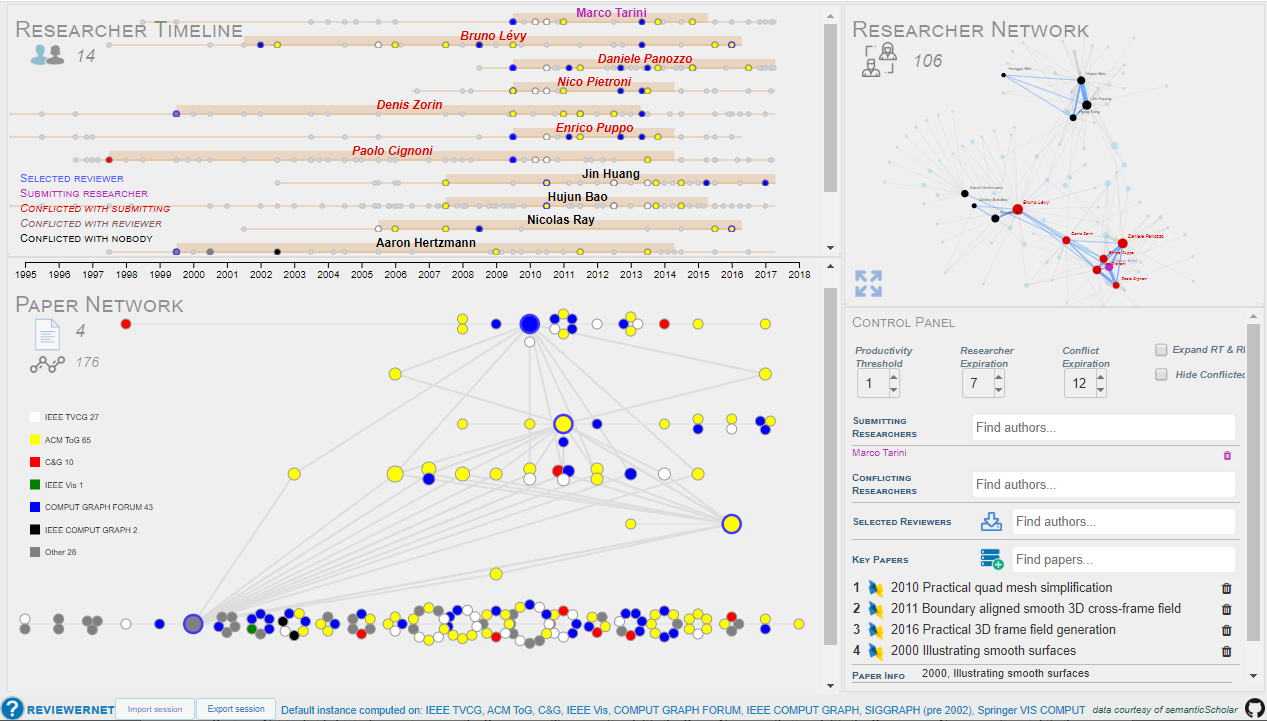
\includegraphics[width=\textwidth]{fig/teaser_colormap2.png}
\caption{The main interface of ReviewerNet, divided into four main areas: the \textsc{Researcher Timeline } (top left); the \textsc{Paper Network }(bottom left); the \textsc{Researcher Network } (top right); the \textsc{Control Panel } (bottom right). The interaction with these areas allows the users to identify researchers working on the topic defined by a network of papers, to analyse the researchers' contributions through time, and to get aware of co-authorship relations and conflicts.}
\label{fig:interface}
\end{figure*}

ReviewerNet supports the various actions that journal editors and IPC members perform while choosing reviewers, namely, searching the literature about the submission topic, looking for active experts in the field, and checking their conflict of interest. ReviewerNet does so by integrating an overview visualization of the literature with a visualization of the career of potential reviewers, their conflict of interests, and their nets of collaborators. This combined visualization helps to make sense of scholarly data, and rapidly get enough understanding to make a sensible decision, as shown in our user study (see Chapter~\ref{sec:evaluation}). 

ReviewerNet integrates the visualization of three main classes of data in a single window (see Figure~\ref{fig:interface}):

\begin{itemize}
\item  {\bf Paper Network} (PN): a chronologically ordered visualization of the literature citation network related with the submission topic. The nodes represent papers, while arcs represent in- and out-citation relations between papers. The horizontal dimension represents time. By means of interactive graph expansion functionalities, the PN supports the rapid exploration of key papers in the literature with respect to the topic of the submitted paper. The authors of the key papers identified will define the set of the candidate reviewers. The PN is built by the users, starting from a small number of seed papers of their choice;
\item  {\bf Researcher Timeline} (RT): a time-based visualization of the academic career of researchers, through horizontal lines and bars. The RT helps assessing the suitability of potential reviewers, showing thier topic coverage, productivity over years, and stage of career. Also, visual cues help the user to tell apart candidate reviewers from conflicting researchers. The RT is built automatically by ReviewerNet while the user builds the PN;
\item  {\bf Researcher Network} (RN), a graph visualization of co-authorship relations: the nodes represent the authors in the PN and their collaborators in the dataset; the arcs connect authors who have publications in common. The aim of the RN is to visualize the research communities: indeed, the identification of network of collaborators helps looking for sets of independent, non-conflicting reviewers. As with the RT, the RN is built online by ReviewerNet.
\end{itemize}
%
The basic pipeline for finding reviewers with ReviewerNet involves: building the Paper Network starting from a small set of seed documents, whose titles are either manually typed, or imported from a list, and automatically parsed and matched in the dataset; evaluating possible choices of reviewers, by navigating the Reviewer Timeline and the Reviewer Network; and finally obtaining a justified list of chosen reviewers, along with possible substitutes suggested by ReviewerNet in case of declined invitation. The user can navigate the different views and interact with the system through simple actions, to drive his/her investigation. Each view in ReviewerNet is linked to the other views, so that so that any action in a view is reflected in the others. Visual cues are used to improve the comprehension during interactive sessions: the position, colour, size, boundary, and style of visual elements visually represent important characteristics of the entities they stand for. To better explain how ReviewerNet works, the next Section presents an example user scenario. %In addition, since a static description may not adequately convey the dynamic nature of the investigation with ReviewerNet, we refer the reader to the accompanying video at \url{https://www.youtube.com/watch?v=JnomPO8QI28}, which illustrates the scenario described below. Finally, 

The technical details about the system are reported in Chapter \ref{sec:impl}.

The user can navigate the different views and interact with the system through simple actions, to drive his/her investigation. Each view in ReviewerNet is linked to the other views, so that so that any action in a view is reflected in the others. Visual cues are used to improve the comprehension during interactive sessions: the colour, size, boundary, and style of visual elements visually represent important characteristics of the entities they stand for. Moreover, the coherence of visual cues across different views enforces their meaningfulness, and makes it easy for the user to switch between different views without losing focus.  

ReviewerNet builds on a reference database including papers, authors and citations from selected sources (journal articles and conference papers) taken from the Semantic Scholar Research Corpus~\cite{ammar:18}. ReviewerNet can be built over any dataset, according to the domain of interest.

\section{Summary of contribution}

My contribution to this thesis is the development and validation of the visualization system, starting from the data gathering and processing. The challenges faced in this process were: dealing with both the size and quality of the corpus and having usable and meaningfull user interface and interactions. I downloaded and processed a Big-Scholarly-Data coprus with simple and reusable scripts, allowing the user to instantiate the platform over any subset of the original corpus with minimum effort (see Chapter \ref{sec:misccode}). 

The main contribution in deployment of the user interface is the resulting layout that allows the user to visualize and interact with all the classes of data visualized at once, thus providing the user with an high number of information about papers, researchers and relationships between them.

The platform has also been validated by a pool of senior researchers in Computer Graphics, who returned positive feedbacks about the ease-of-use and the distribution and quality of the candidate reviewers found using ReviewerNet, along with suggestion for further improvements (see Chapter \ref{sec:evaluation}). 

The tool is open, and the source code is available at~\url{https://github.com/cnr-isti-vclab/ReviewerNet}, while the demonstration platform is available at~\url{https://reviewernet.org}.
\section{Outline}

In the next Chapter \ref{sec:related}, we review state-of-the-art applications and methods built on top of scholarly data.

Then, we define our goals and use-case along with the notation that is used in the document, along with a detailed description  (Chapter~\ref{sec:platform}). 

We describe how the user interface is composed and the possible interactions the user can exploit during the reviewer selection (Chapter~\ref{sec:userinterface}). 

We demonstrate the platform in the field of Computer Graphics and show how ReviewerNet can be used to search for reviewers who are expert on a certain topic, are at a certain career stage, who have a certain track of publishing records, who are not conflicting with neither the submitters nor other reviewers, and who are well-distributed in the scientific community (Chapter~\ref{sec:demonstration}). 

We evaluate the platform through a user study involving 15 real end-users from the Computer Graphics community and show how they were able to get acquainted with ReviewerNet even with very limited training, and how they rated very positively ReviewerNet functionalities (Chapter~\ref{sec:evaluation}).  

We then conclude with a discussion on the main contributions of this thesis and further imporovements to the system (Chapter \ref{sec:conclusions}).

\section{Publications}

A preliminary version of the platform developed for this thesis was presented at the 2019 edition of the Smart Tools and Applications in Graphics conference \cite{stag19}, where the paper earned the \virgolette{\emph{Best Paper}} nominee and was selected for publication ia a \emph{Special Issue} of the Elsevier Computers \& Graphics journal. The newly submitted paper is currently under review.

\section*{Acknowledgments}

The authors would like to thank the Allen Institute for Artificial Intelligence for providing the Semantic Scholar corpus of bibliographic data.